\documentclass[12pt, a4paper]{article}
\usepackage[margin=2.5cm]{geometry}
\usepackage[utf8]{inputenc}
\usepackage{color, amssymb}
\usepackage{listings, amsmath, float}
\renewcommand{\baselinestretch}{1.5}
\setlength\parindent{24pt}
\usepackage{graphicx}
\graphicspath{ {./images/} }

\title{Lab 2}
\author{Odysseas Stavrou}
\date{November 2020} 

\begin{document}
\noindent\rule{\textwidth}{1.5pt}

\begin{center}
{\bf Digital Signal Processing} \\ 
 2nd Lab Exercise\\
 Odysseas Stavrou 2018030199\\
 Lab Group No: 90\\
 November 2020\\
 Technical University of Crete\\
\end{center}
\noindent\rule{\textwidth}{1.5pt}

\begin{enumerate}
    \item[1.] Given the following system arragement:
    \[k(n) = 0.9k(n-1) + 0.2x(n)\]
    \[G_2(z) = \frac{1}{z + 0.2}\]
    \begin{figure}[H]
        \centering
        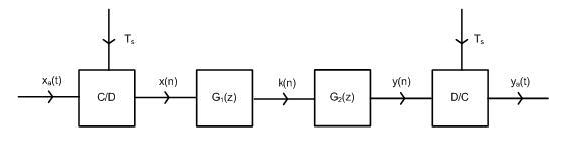
\includegraphics[width=\textwidth]{1.png}
    \end{figure}
    \begin{enumerate}
        \item[a.] Find the transfer function \(H(z)\) of the system and also the difference equation
        for input/output:
        \begin{enumerate}
            \item[i.] Apply the Z-Transfom on \(k(n)\):
            \[Z_n[k(n)] \Rightarrow K(z) = 0.9z^{-1}K(z) + 0.2X(z)\qquad(1)\]
            \item[ii.] Rearraning \((1)\) we can derrive \(G_1(z)\):
            \[K(z)(1-0.9z^{-1}) = 0.2X(z)\]
            We know:
            \[G_1(z) = \frac{K(z)}{X(z)} = \boxed{\frac{0.2z}{z-0.9}}\]
            \item[iii.] The transfer function is the product of \(G_1(z)\cdot G_2(z)\):
            \[H(z) = \frac{0.2z}{z-0.9}\cdot \frac{1}{z+0.2} = \boxed{\frac{0.2z}{z^2 - 0.7z - 0.18}}\]

            \item[iv.] The transfer function is the relation between the output and the input:
            \[H(z) = \frac{Y(z)}{X(z)}\]
            \[\frac{0.2z}{z^2 - 0.7z - 0.18} = \frac{Y(z)}{X(z)}\]
            Multiplying cross-wise we get:
            \[z\cdot Y(z) - 0.7\cdot Y(z) - 0.18 \cdot z^{-1} \cdot Y(z) = 0.2 \cdot X(z)\]
            Using the following propery we can easily derrive the Inverse Z.T.:
            \[Z_n[x(n - n_0)] \rightleftarrows z^{-n_0} X(z)\]
            Inverse Z.T.:
            \[y(n+1) - 0.7y(n) - 0.18y(n-1) = 0.2x(n)\]
            \[\boxed{y(n) = -\frac{2}{7}x(n) -\frac{9}{35}y(n-1) + \frac{10}{7}y(n+1)}\]
        \end{enumerate}
        \item[b.] Plot the Poles and Zeroes of the T.F. using MATLAB's \textbf{tf} and \textbf{zplane} functions:
        \begin{figure}[H]
            \centering
            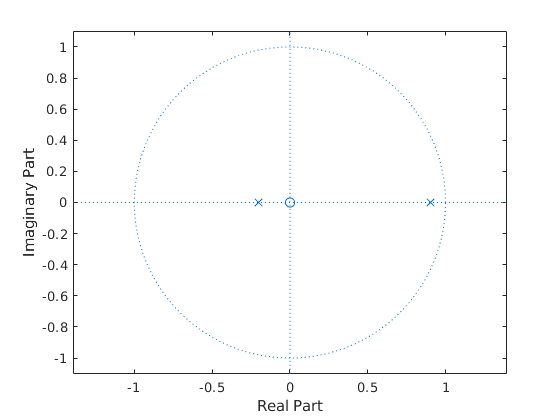
\includegraphics{zplane.png}
        \end{figure}
        \item[c.] A casual system is stable if all the poles fall into the Unit Circle, something that in this case holds. So the system is stable
        \item[d.] Plotting the frequency response:
        \begin{figure}[H]
            \centering
            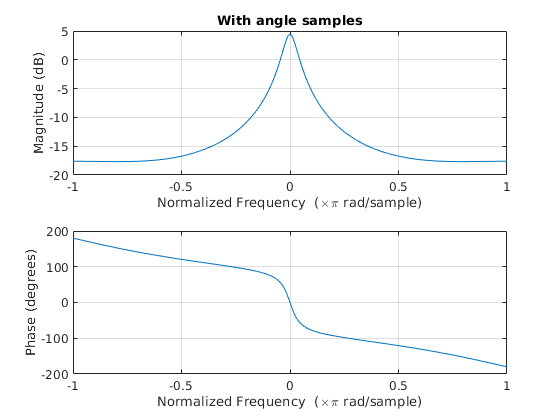
\includegraphics[scale=0.9]{ANG.png}
            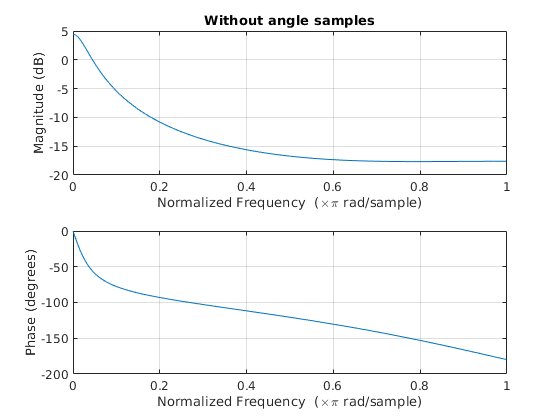
\includegraphics[scale=0.9]{no_ANG.png}
            \caption{Frequency response with and without angle samples}
        \end{figure}
        \begin{itemize}
            \item Comparing the two figures we observe that by not having the angle samples the graph depicts only the right (positive) part of the graph, thus we can not observe
            the symmetry.
        \end{itemize}
        \item[e.] Adding one more Pole \(z = 1\) to \(H(z)\):
        \[H(z) = \frac{0.2z}{(z-0.9)(z+0.2)}\]
        Adding new Pole \(z = 1\)
        \[H(z) = \frac{0.2z}{(z-0.9)(z+0.2)(z - 1)}\]
        Simplify:
        \[H(z) = \frac{0.2z}{z^3 - 1.7z^2 + 0.52z + 0.18}\]

        \begin{figure}[H]
            \centering
            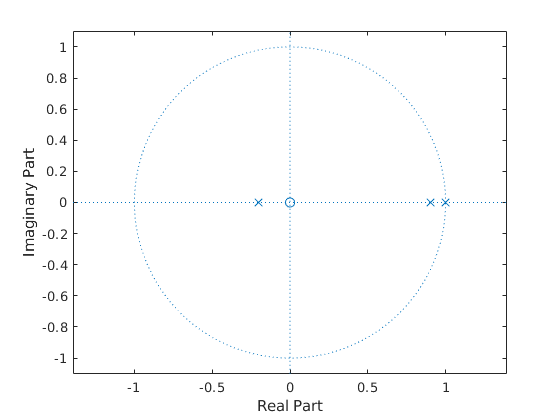
\includegraphics[scale=0.9]{new_pole.png}
            \caption{Zplane of \(H(z)\) with the added Pole}
        \end{figure}

        \begin{figure}[H]
            \centering
            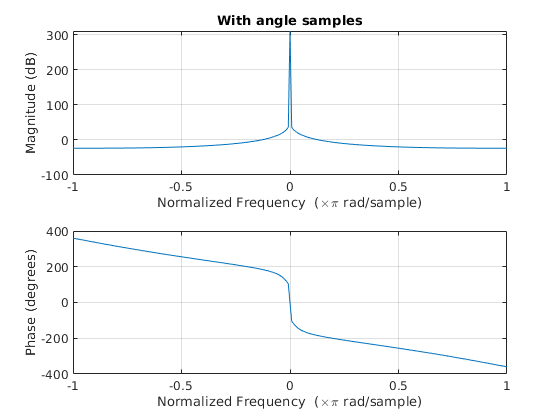
\includegraphics[scale=0.9]{new_pole_freqz.png}
            \caption{Frequency response of \(H(z)\) with the added Pole}
        \end{figure}

        \begin{itemize}
            \item Adding one more Pole to the T.F. reduces the response time
            \item The phase shift is doubled and way more steep than in 1.d
            \item The closer the Poles are to the Unit Circle, the higher the amplification and the more selective the Frequencies become,
            that is why we see a sharp spike
        \end{itemize}
        
    \end{enumerate}
    \item[2.] Given the following Transfer Function:
    \[H(z) = \frac{4-3.5z^{-1}}{1-2.5z^{-1}+z^{-2}}\quad ,|z| > 2\]
    \begin{enumerate}
        \item[a.] Using MATLAB (\textbf{syms, residuez, pretty} functions) decompose \(H(z)\) into fractions:\\
        The decomposed Transfer Function results in 2 fractions:
        \[H_1 = -\frac{3z}{2-z} = \boxed{\frac{3z}{z-2}}\]
        \[H_2 = -\frac{2z}{1 - 2z} = -\frac{z}{\frac{1}{2} - z} = \boxed{\frac{z}{z-\frac{1}{2}}}\]
        \item[b.] By using the Z.T. propery:
        \[Z_n[k_i a^n \cdot u[n]] \rightleftarrows \frac{k_i z}{z-a}\]
        We can calculate the Inverse Z.T. of each fraction:
        \[h{[n]}_1 = Z_n^{-1}[H_1] = Z_n^{-1}\left[\frac{3z}{z-2}\right] = \boxed{3\cdot2^n \cdot u[n]}\]
        \[h{[n]}_2 = Z_n^{-1}[H_2] = Z_n^{-1}\left[\frac{z}{z-\frac{1}{2}}\right] = \boxed{\frac{1}{2}^n \cdot u[n]}\]
        \newline
        The resulting Inverse Z.T. is the sum of \(h{[n]}_1 + h{[n]}_2\):
        \[\boxed{h[n] = 3\cdot2^n \cdot u[n] + \frac{1}{2}^n \cdot u[n]\quad ,|z| > 2}\]
        This is also confirmed using MATLAB's \textbf{iztrans} function:
        \begin{figure}[H]
            \centering
            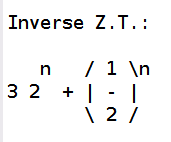
\includegraphics[scale=0.6]{izt.png}
            \caption{Inverse Z.T. oh \(H(z)\)}
        \end{figure}
    \end{enumerate}
\end{enumerate}

\end{document}